\documentclass{article}
\usepackage[pdfcreator={LaTeX}]{hyperref}
\usepackage{graphicx}
\usepackage[utf8]{inputenc} 
\usepackage[ngerman]{babel}

\usepackage[section,toc]{glossaries}\makeglossaries

\newglossaryentry{Regelwerk}{name=Regelwerk,
	plural = Regelwerke,
	description={Regeln eines bestimmten Kartenspiels}
}
\newglossaryentry{Client}{name=Client,
	plural = Clients,
	description={Der Benutzer einer Applikation}
}
\newglossaryentry{Server}{name = Server,
	description={Rechner,der Dienste zur Verfügung stellt}
}
\newglossaryentry{Lobby}{name = Lobby,
	description={Ort, an dem Spieler ein Kartenspiel auswählen oder beitreten können}
}
\newglossaryentry{GUI}{name = GUI,
	description={Graphische Oberfläche}
}
\newglossaryentry{Spielleiter}{name = Spielleiter,
	description={Derjenige, der in der Lobby ein neues Spiel erstellt}
}
\newglossaryentry{akkumuliert}{name = akkumuliert,
	description={Gehäuft, nicht einzeln}
}

\begin{document}
\begin{titlepage}

\begin{center}
\textbf{\textsc{\LARGE Pflichtenheft}}

{\large \today}

\vspace{2cm}
\includegraphics{Bild}

\vspace{2cm}

\begin{tabular}{|c|c|c|}\hline
   Phase & Verantwortlicher & E-Mail \\ \hline\hline
   Pflichtenheft & Alina  Meixl  &  alina@meixl.de \\ \hline
   Entwurf & Viktoria Witka & witkaviktoria@freenet.de \\ \hline
   Spezifikation & Daniel Riedl & dariedl14@yahoo.de \\ \hline
   Implementation & Andreas Altenbuchner& a.andi007@gmail.com\\ \hline
   Verifikation &Patrick Kubin & kubin@fim.uni-passau.de\\ \hline
   Präsentation & w& w\\ \hline
 \end{tabular}

\end{center}

\end{titlepage}


\tableofcontents

\section{Zielbestimmung}
Ein Online-Multiplayer Kartenspiel.

\subsection{Musskriterien}
Es gibt einen \gls{Server} der das Spiel verwaltet und \glspl{Client} die spielen.
\subsubsection{\gls{Server}}
\begin{itemize}
	\item \glspl{Client} können sich verbinden und eindeutigen Benutzernamen auswählen
	\item \gls{Lobby} mit der Möglichkeit, Spiele zu erstellen und offenen Spielen beizutreten
	\item Unterstützung mehrere parallel laufender Spiele
	\item Regelauswertung mit Überprüfung erlaubter Aktionen, Punktezählung, Kartenausgabe
	\item Unterstützung der Spiele Hearts und Wizard
	\item Chat in der \gls{Lobby}
	\item Chat mit Mitspielern während eines Spiels
	\item Schutz vor Cheats (Mehrfachanmeldung?)
\end{itemize}

\subsubsection{\gls{Client}}
\begin{itemize}
	\item GUI
	\begin{itemize}
		\item Darstellungsfenster, das mindestens bei der Auflösung von 1024x768 Bildpunkten benutzt werden kann
		\item Darstellung des laufenden Spiels (eigene Hand, verdeckte Hand der anderen Spieler, Ablage- und Aufnahmestapel, 			Punktestand, evtl. Zusatzinformationen)
		\item Eingabemöglichkeiten für erlaubte Aktionen während des Spiels (Karte ablegen, Ansagen, etc.)
		\item Die \gls{GUI} muss den Benutzer sinnvoll unterstützen und benutzerfreundliche Eingabeelemente anbieten
		\item Flüssige Darstellung
		\item Unabhängigkeit vom \gls{Regelwerk}
		\item Beim Start Auswahl des \gls{Server}s und des Benutzernamens
		\item Anzeige von offenen Spielen in der \gls{Lobby} mit Möglichkeit zum Erstellen und Beitreten
		\item Chat in der \gls{Lobby} und während des Spiels
	\end{itemize}
	\item Modell
	\begin{itemize}
		\item Verwaltung der Verbindung mit dem \gls{Server}
		\item Verwaltung des aktuellen Spielzustands (soweit \gls{Client} bekannt)
		\item Vorab-Regelauswertung zur Unterstützung des Nutzers (ungültige Spielaktionen sind nicht durchführbar in der 					\gls{GUI})
	\end{itemize}
\end{itemize}

\subsection{Wunschkriterien}
\begin{itemize}
	\item Weitere \glspl{Regelwerk} (Uno, Mau-Mau, Black Jack)
	\item Scoresystem
	\item Statistiken
	\item Mehrsprachen
	\item Veränderbare \gls{GUI} (Farben etc)
\end{itemize}

\subsection{Abgrenzungskriterien}
\begin{itemize}
	\item Beitreten eines bereits laufenden Spieles nicht möglich.
	\item keine Persistenz über mehrere Sessions, keine Registrierung
	\item keine KI
\end{itemize}

\section{Produkteinsatz}
\subsection{Anwendungsbereich}
Internetspiel im Freundeskreis.
\subsection{Zielgruppe}
Personen, die gemeinsam über ein lokales Netzwerkoder das Internet spielen möchten. 
\subsection{Betriebsbedingungen}
Betriebsdauer ?

\section{Produktumgebung}
\subsection{Software}
	\begin{itemize}
		\item \gls{Client}
		\begin{itemize}
			\item ...
		\end{itemize}
		\item \gls{Server}
		\begin{itemize}
			\item ...	
			\item ...
		\end{itemize}
	\end{itemize}

\subsection{Hardware}
\begin{itemize}
		\item \gls{Client}
		\begin{itemize}
			\item Internetfähiger Rechner
		\end{itemize}
		\item Server
		\begin{itemize}
			\item Internetfähiger Rechner	
			\item Speicherplatz
			\item Rechenleistung
		\end{itemize}
	\end{itemize}

\subsection{Orgware}
Internetverbindung.

\section{Produktfunktionen}
\subsection{Startseite}
\begin{itemize}
	\item /F040/ Auswahl vom gewünschtem \gls{Server} und Namen, danach Weiterleitung zur \gls{Lobby}
	\item /F050W/ Auswahl der Sprache
\end{itemize}

\subsection{\gls{Lobby}}
\begin{itemize}
	\item /F060/ Anzeige von eingeloggten Spieler
	\item /F070/ Chatten mit anderen eingeloggten Spielern auf dem \gls{Server}
	\item /F080/ Anzeige offener Spiele mit Spielart und Spieleranzahl sowie die Option den Spielen beizutreten (Weiterleitung zum Wartefenster)
	\item /F090/ Option ein eigenes Spiel zu erstellen(Weiterleitung zum Erstellungsfenster)
	\item /F100/ Hilfe zu den Spielarten
\end{itemize}

\subsection{Erstellungsfenster}
\begin{itemize}
	\item /F120/ Auswahl vom \gls{Regelwerk} und  Namen des Spiels 
	\item /F130W/ Möglichkeit ein Passwort für das Spiel zu setzen
\end{itemize}

\subsection{Passwortabfrage}
\begin{itemize}
	\item /F140/ Abfragen des vom Host gewählten Passworts
	\item /F142/ Zugang zum Wartefenster gewähren
	\item /F145/ Abbrechen und zur Lobby zurückkehren
\end{itemize}

\subsection{Wartefenster}
\begin{itemize}
	\item /F150/ Anzeigen des Spieltyps, der Spieler und Spielerzahl
	\item /F160/ Ab Mindestanzahl der Spieler kann der Spielersteller des Spiel starten
	\item /F170/ Wartefenster wird nur aufgelöst wenn der Spielersteller selbst das Spiel verlässt
	\item /F180/ Spielleiter kann unerwünschte Spieler entfernen
\end{itemize}

\subsection{Spiel}
\begin{itemize}
	\item /F190/ Anzeige des Spiels, der eigen Karten, der verdeckten Karten der Mitspieler sowie Ablage-und Aufnahmestapel
	\item /F200/ Anzeige von Punktestand oder anderen Zusatzinformationen
	\item /F210/ Eingabemöglichkeit für regelkonforme Aktionen
	\item /F220/ Chatten mit anderen Mitspielern
	\item /F230/ Wenn einer das Spiel verlässt wird das Spiel beendet und die anderen Mitspieler werden zur \gls{Lobby} zurückgeleitet
	\item /F240/ Hilfe zu dem Spiel
	\item /F250/ Auswertung bei Ende des Spiels
\end{itemize}

\section{Produktdaten}

\begin{itemize}
	\item /D010/ \gls{Lobby}daten
	 \begin{itemize}
	 	\item Spielerdaten
	 	\begin{itemize}
	 		\item Spielername(eindeutig)
	 	\end{itemize}
	 	\item Spieledaten
	 	\begin{itemize}
	 		\item Spielenamen(eindeutig)
	 		\item Spieltyp
	 		\item Anzahl an Spielern und maximale Anzahl an Spielern
	 	\end{itemize}
	 \end{itemize}
	 \item /D020/ Erstellungsdaten
	 \begin{itemize}
	 	\item \gls{Spielleiter}(eindeutig)
	 	\item Spielernamen(eindeutig)
	 	\item Spieleranzahl und maximale Spieleranzahl
	 	\item Spieltyp
	 	\item Mindestanzahl an Spielern erreicht
	 \end{itemize}
	 \item /D030/ Spieldaten
	 \begin{itemize}
	 	\item Spielname(eindeutig)
	 	\item Spieltyp
	 	\item Anzahl an Spielern
	 	\item Kartenstapel
	 	\begin{itemize}
	 		\item Anzahl verbliebener Karten
	 		\item Karten
	 		\item Ausgabe von Karten
	 	\end{itemize}
	 	\item Zugreihenfolge
	 	\item Spieler
	 	\begin{itemize}
	 		\item Name(eindeutig)
	 		\item Kartenhand
	 		\begin{itemize}
	 			\item Karten
	 			\item Anzahl
	 			\item Spielbar
	 		\end{itemize}	 
	 		\item Bedenkzeit(X minuten)		
	 	\end{itemize}
	 	\item Punktestand und Siegbedingung
	 \end{itemize}
\end{itemize}

\section{Produktleistungen}
\begin{itemize}
	\item /L040/ Einhaltung der Spielregeln gewährleisten
	\item /L050/ Fehlermeldungen \gls{akkumuliert} ausgeben
	\item /L060/ Verwaltung mehrerer parallel laufender Spiele
	\item /L070/ Chat und Spiel sollen flüssig laufen
	\item /L080/ Einfache und hilfreiche Bedienbarkeit
	\item /L090/ Schutz vor Cheats
	\item /L100/ Verhinderung langer Wartezeiten
	\item /L110W/ Mehrsprachigkeit unterstützen
\end{itemize}

\section{Benutzungsoberfläche}
\begin{itemize}
	\item Startseite: \\ 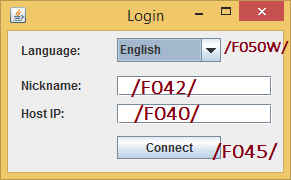
\includegraphics{GUI_images/Login}
	\item Lobby: \\ 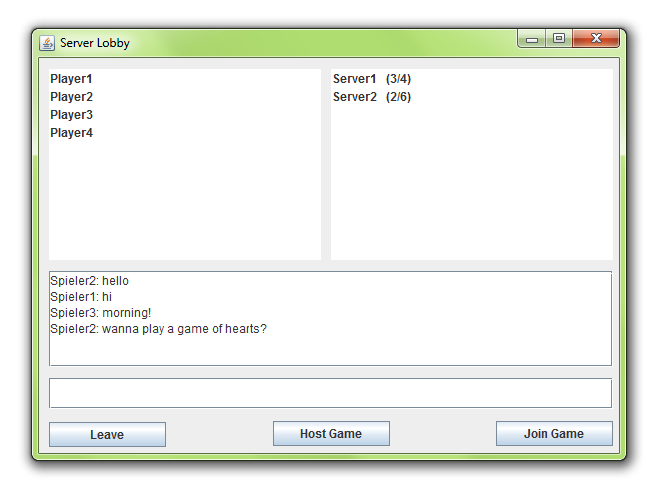
\includegraphics[scale=0.7]{GUI_images/ServerLobby}
	\item Erstellungsfenster: \\ 
		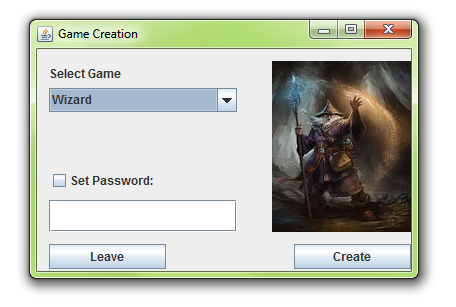
\includegraphics[scale=0.8]{GUI_images/CreateGame}
	\item Wartefenster: \\ 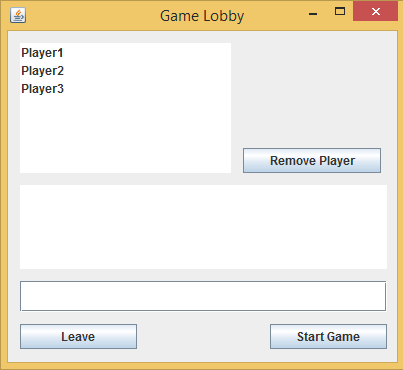
\includegraphics[scale=0.7]{GUI_images/GameLobby}
	\item Passwortabfrage: \\ 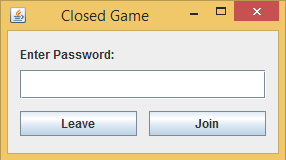
\includegraphics{GUI_images/PasswordRequest}
	\item Spiel: \\ 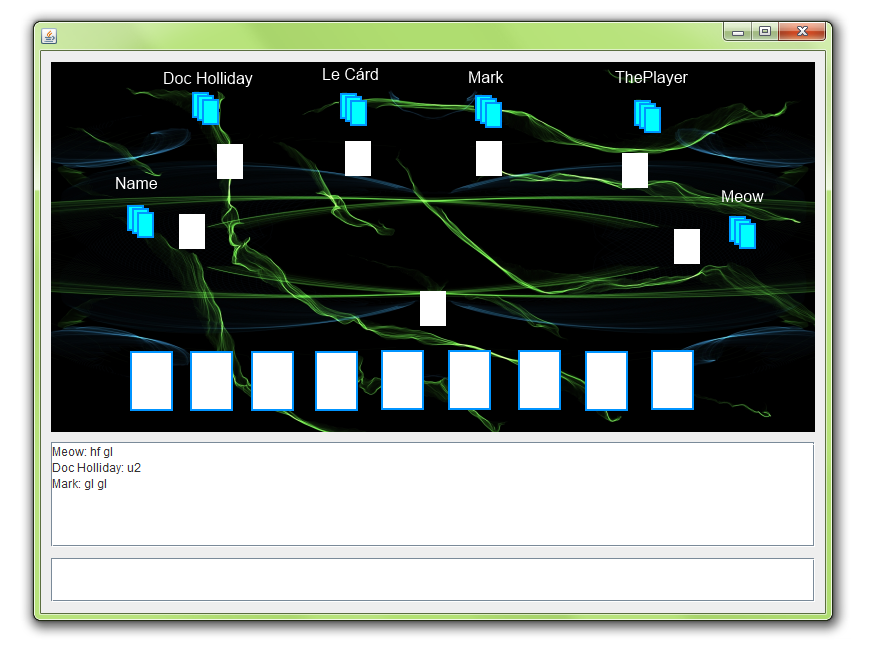
\includegraphics[scale=0.6]{GUI_images/GameClient}
\end{itemize}

\section{Testszenarien}
\begin{itemize}
	\item Benutzername, Server aussuchen
	\item Spiel erstellen (Lobby)
	\item Spiel beitreten (Lobby)
	\item Mehrere Spiele parallel starten (Lobby)
	\item Spiel spielen 
\end{itemize}

\section{Entwicklungsumgebung}
\subsection{Software}
\begin{itemize}
	\item LaTeX
	\item Eclipse 3.8
	\item IBM Rational Software Architect 8.0
	\item .....
\end{itemize}

\subsection{Hardware}
\begin{itemize}
	\item Rechner im CIP Pool	
	\item Private Rechner
\end{itemize}

\subsection{Orgware}
Keine.

\section{Ergaenzung}
..... 
\newpage
\printglossaries
\end{document}
